\documentclass[10pt,twocolumn,letterpaper]{article}

\usepackage{cvpr}
\usepackage{times}
\usepackage{epsfig}
\usepackage{graphicx}
\usepackage{amsmath}
\usepackage{amssymb}
\usepackage{booktabs}
\usepackage{array}
\usepackage{subcaption}
\usepackage{optidef}
\usepackage{xcolor}
\usepackage{tabularx}
\graphicspath{{./img/}}


% \makeatletter
% \@namedef{ver@everyshi.sty}{}
% \makeatother
% \usepackage{tikz}

\usepackage{alphalph}
\renewcommand*{\thesubfigure}{%
\alphalph{\value{subfigure}}%
}%

% \usepackage{alphalph}
% \renewcommand\thesubfigure{\alphalph{\value{subfigure}}}
\renewcommand{\vec}[1]{\mathbf{#1}}
\newcommand{\Real}[1]{\mathbb{R}^{#1}}
\newcommand{\ReLU}{\texttt{ReLU}\,}
\newcommand{\ReLUBN}{\texttt{ReLU + BN}\,}
\newcommand{\moons}{\texttt{MOONS}\,}
\newcommand{\cifar}{\texttt{CIFAR-10}\,}
\newcommand{\SepConstraint}{\texttt{Sep-Cons}\,}
\newcommand{\SepUnit}{\texttt{Sep-U}\,}
\newcommand{\SepLayer}{\texttt{Sep-L}\,}
\newcommand{\SepPoint}{\texttt{Sep-P}\,}
\newcommand{\SepLayerBN}{\texttt{Sep-L-BN}\,}
\newcommand{\SepUnitPoint}{\texttt{Sep-P+U}\,}
\newcommand{\layer}{\ell}
\newcommand\fuck[1]{\textcolor{red}{#1}}
\DeclareMathOperator*{\argmin}{arg\,min}
\DeclareMathOperator*{\argmax}{arg\,max}

% Include other packages here, before hyperref.

% If you comment hyperref and then uncomment it, you should delete
% egpaper.aux before re-running latex.  (Or just hit 'q' on the first latex
% run, let it finish, and you should be clear).
\usepackage[pagebackref=true,breaklinks=true,letterpaper=true,colorlinks,bookmarks=false]{hyperref}

% \cvprfinalcopy % *** Uncomment this line for the final submission

\def\cvprPaperID{6485} % *** Enter the CVPR Paper ID here
\def\httilde{\mbox{\tt\raisebox{-.5ex}{\symbol{126}}}}

% Pages are numbered in submission mode, and unnumbered in camera-ready
\ifcvprfinal\pagestyle{empty}\fi


%%% theorem styles and stuff
\newtheorem{theorem}{Theorem}[section]
\newtheorem{corollary}{Corollary}[theorem]
\newtheorem{lemma}[theorem]{Lemma}
\newtheorem{remark}[theorem]{Remark}
\newtheorem{definition}{Definition}[section]
\newtheorem{proposition}[theorem]{Proposition}

\title{Separation Constraints and Zero Initialization to disencumber Deep Neural Networks}

\author{Riera-Molina C.\\
Universitat de Barcelona\\
Gran Via de les Corts Catalanes 585, Barcelona Spain, 08005\\
{\tt\small blauigris@gmail.com}
% For a paper whose authors are all at the same institution,
% omit the following lines up until the closing ``}''.
% Additional authors and addresses can be added with ``\and'',
% just like the second author.
% To save space, use either the email address or home page, not both
\and
Rey-Torres C.\\
Universitat de Barcelona\\
Gran Via de les Corts Catalanes 585, Barcelona Spain, 08005\\
{\tt\small camilorey@gmail.com}
}
\begin{document}
\maketitle
\begin{abstract}
The large variety of techniques available to facilitate deeper Neural Networks add complexity to the design process. In this work we simplify those decisions by introducing a set of constraints that attempts to replace them. Through a geometrical formulation we develop a set of constraints that force the units to perform separations on the data. This has the effect of linking the internal representations generated while transforming input to output, in favor of the back-propagation. The resulting network produces more \emph{intuitive} outputs, has greater representational power, reduces vanishing gradient and dead units, and allows Zero Initialization. Visual assessment of the effect of the separation constraints is provided through experimentation (contrasted to Batch Normalization), constructing insights from the results of our theoretically grounded geometrical framework. 
\end{abstract}

\section{Introduction}\label{sec:introduction}

% Párrafo introductorio
The success of Deep Learning has traditionally been linked to its ability to learn \emph{abstract representations} of data using function composition\cite{LeCun06atutorial}. These functions (i.e. the \emph{layers}) decompose and solve the problem in \emph{parts} \cite{resnetSubtree} profiting their feed-forward structure \cite{backprop}. However, the deeper the network, the more susceptible it becomes to issues affecting backpropagation as a learning strategy \cite{backprop} (e.g. the vanishing gradient problem, \cite{vanishing1,vanishing2} the exploding gradient \cite{exploding} and the dead unit problem \cite{leaky,whyreludie,whenneuronsfail}) . 
\\\\
% Problema general
There are \emph{essentially} two families of methods to address these issues: \emph{architectural modifications} to the network and input data \emph{manipulation}. Examples of architectural modifications include (1) layer-width increase as done in \cite{wideresnet,inceptionv1}; (2) feed-forward structure network modification, as done in ResNets \cite{resnet} or DenseNets \cite{densenet}; (3) unit based alterations (of the their non-linearity or activation) as done in \emph{leaky}-\ReLU \cite{leaky} or \texttt{PReLU} \cite{prelu}). Meanwhile, the most commonly used data manipulation technique is \emph{data normalization} techniques on the output of layers as done under \emph{batch normalization} \cite{batchnorm}.  
\\\\
For example, layer-width increases reduces the chance for \emph{useless} units (e.g. dead or \emph{redundant}) per layer. However, such measures increase the computational cost of the network and the dimensionality of the problem, hampering convergence \cite{cursedim} and taking a toll on speed. Meanwhile, modifying network connectivity may prove beneficial to tackle the vanishing gradient \cite{ladder,nin,highway}. This occurs however, at the expense of burdening designers with additional \emph{architectural} decisions (e.g. which connection to add or alter) taking a toll in parameter and hyper-parameter number as presented for example in \cite{densenet}. 
\\\\
In turn, unit activation modification intends to ensure non-zero gradient back-propagation by (1) modifying unit functions to avoid zero truncation as done in \cite{leaky}, \cite{prelu}, \cite{elu} or \cite{selu} (\ReLU modifications) or modifying unit output \cite{crelu}. With batch normalization \cite{batchnorm}, several drawbacks have been described in works like \cite{batchrenorm} and \cite{batchnormGradientExplosion}: decreased performance in testing due to non-matching statistical parameters between training and testing (e.g. mean value and variance or non-i.i.d. minibatches or small batch sizes \cite{batchrenorm}; and exploding gradients limiting the depth of the network \cite{batchnormGradientExplosion}.
\\\\
% Problema específico (Pregunta del paper)
Since existing methods require either computational expenditure and add arbitrary complexity to the architecture design, or simply entail limit network performance, we wonder whether we can train deeper networks without relying in any of those techniques. This imply using the minimum width possible, removing any additional connections or activations, and using no normalization. 
\\\\
We argue that those problems can be tackled at unit level, since they stem from the affine/dead unit problem. In this sense, we argue that 
affine unit \emph{downgrades} the unit to an redundant transform (since it can be carried out by the following unit), \emph{dead} units compromise the \emph{representative} ability of the network.
\\\\
While dead neurons have been traditionally accepted as a minor issue for DNN related phenomena, affine units are not usually seen as hazardous are also not devoid of caveats.
\\\\
% Solución propuesta (Respuesta a la pregunta)
We propose to achieve that by introducing a family of constraints which increase the separation performed by each of the units on the data. We demonstrate that doing so helps in avoiding trivial failure modes like dead or linear units. Additionaly, enables the use of zero initialization. The only added cost is an additional loss per layer and the inclusion of an additional hyperparameter. 
\\\\
% Estructura del paper
This paper is organized as follows: section \ref{sec:separability} motivates the importance of enforcing separation in the units), after that section presents the \ref{sec:constraint} the actual constraints that we impose on the network to do so. Section \ref{sec:experiments} provides with experimental interpretation of the effect of the constraints and finally section \ref{sec:conclusions} closes the paper with the main conclusions.

\begin{table*}[h!]
    \centering
\begin{tabular}{@{}llll@{}}
\toprule
Family                         & Method                                                             & Examples                                                                                                                                                                                                                                                   & Intended issues                                                                \\ \midrule
\multirow{3}{*}{Architectural} & Width increase                                                     & \begin{tabular}[c]{@{}l@{}}Wide \textbackslash{}texttt\{ResNet\} \textbackslash{}cite\{wideresnet\}\\ \textbackslash{}texttt\{Inception\} \textbackslash{}cite\{inceptionv1\}\end{tabular}                                                                 & \begin{tabular}[c]{@{}l@{}}Vanishing Gradient\\ Increase Depth\end{tabular}    \\
                               & \begin{tabular}[c]{@{}l@{}}Connection \\ modification\end{tabular} & \begin{tabular}[c]{@{}l@{}}\textbackslash{}texttt\{ResNet\} \textbackslash{}cite\{resnet\} \\ \textbackslash{}texttt\{DenseNet\} \textbackslash{}cite\{densenet\}\end{tabular}                                                                             & \begin{tabular}[c]{@{}l@{}}Vanishing Gradient\\ \\ Increase Depth\end{tabular} \\
                               & Unit Alteration                                                    & \begin{tabular}[c]{@{}l@{}}\textbackslash{}emph\{leaky\}-\textbackslash{}ReLU \textbackslash{}cite\{leaky\} \\ \textbackslash{}texttt\{PReLU\} \textbackslash{}cite\{prelu\}\\ \textbackslash{}texttt\{C-ReLU\} \textbackslash{}cite\{crelu\}\end{tabular} & \begin{tabular}[c]{@{}l@{}}Vanishing Gradient\\ Dead Neurons\end{tabular}      \\
Data Manipulation              & Modify layer output                                                & \textbackslash{}emph\{batch normalization\} \textbackslash{}cite\{batchnorm\}                                                                                                                                                                              & Exploding Gradient                                                             \\ \bottomrule
\end{tabular}
\end{table*}

\section{\ReLU Based Separation}\label{sec:separability}
A classical feed-forward DNN $F$ can be formally approached as a multi-valued real function $F(\vec{x})$, that is created by composing a collection of vector \emph{layer} functions $\layer:\Real{n_k}\rightarrow\Real{n_{k+1}}$. The hidden layers are defined as the sum of collection of scalar functions dubbed as the \emph{units}: 
\begin{equation}\label{eq:layer}
\layer_k(\vec{x}) = \sum^{n_{k+1}}_{j=1} u_i^k(\vec{x}) \hat{\textbf{e}}_i
\end{equation}
that depend on a weight vector $\vec{w}_j^k\in\Real{n_k}$ and a bias parameter $b_j^k\in\mathbb{R}$ affinely, featuring a truncation on negative values:
\begin{equation}\label{eq:unit}
u_j^k(\vec{x}) = \max\{0,\vec{w}_j^k \cdot \vec{x} + b_j^k\}
\end{equation}
it is trivial to see that each unit defines a partition of the space $\Real{n_k}$ in two sets\footnote{Compare to the \emph{acceptance} and \emph{denial} zones in Rey-Torres et al. \cite{reyRiera2019ModellingClassificationReLU}}: the \emph{upper} part of unit $u_j^k$ and the \emph{lower} part of $u_j^k$:
\begin{equation}\label{eq:upperAndLowerSets}
\begin{array}{lcl}
    upper(u_j^k) &=& \{\vec{x}:\vec{w}_j^k \cdot \vec{x} + b_j^k > 0\}\\\\
    lower(u_j^k) &=& \{\vec{x}:\vec{w}_j^k \cdot \vec{x} + b_j^k\leq 0\}\\
\end{array}
\end{equation}
We define $upper(u_j^k)$ as the positive half-space of the plane 
\begin{equation}\label{eq:separatingPlane}
    \Pi(\vec{w}_j^k,b_j^k) = 
    \{ 
     \vec{x}:\vec{w}_j^k\cdot\vec{x}+b_j^k =0
    \}
\end{equation}
while $lower(u_j^k)$ corresponds to the closure of its negative half-space. Based on Rey-Torres et al. \cite{reyRiera2019ModellingClassificationReLU}, we define the \emph{affine} component of a layer function $\layer_k$ as the intersection of the upper parts of its units, and its zero set correspondingly:
\begin{equation}\label{eq:affineCompAndZeroSet}
\begin{array}{cc}
    A(\layer_k) = \displaystyle\bigcap_{j=1}^{n_{k+1}}upper(u_j^k), &
    Z(\layer_k) = \displaystyle\bigcap_{j=1}^{n_{k+1}}lower(u_j^k)\\
    \end{array}
\end{equation}
both $A(\layer_k)$ and $Z(\layer_k)$ are convex open polytopes in $\Real{n_k}$ not necessarily bounded \cite{florenzano2001ConvexAnalysis,reyRiera2019ModellingClassificationReLU}, so that their complement is a closed non-convex set: the \emph{interzone} of $\layer_k$, that corresponds to the region of $\Real{n_k}$ that is neither forwarded affinely nor is mapped to zero \footnote{Compare to the \emph{ambiguity zone} of \cite{reyRiera2019ModellingClassificationReLU}}:
\begin{equation}\label{eq:interzone}
    I(\layer_k) = \Real{n_k}\setminus(A(\layer_k)\cup Z(\layer_k))
\end{equation}
an important fact to keep in mind with regards to \ReLU based DNN is that the output of layers features exclusively vectors with non-negative components. In this sense, $\layer_k$ maps $\Real{n_k}$ into the first hyperoctant of $\Real{n_{k+1}}$.
Thus, $\layer_k$ defines a mapping into $\Real{n_{k+1}}_{+}$ such that: 
\begin{itemize}
    \item it maps the affine component into the \emph{interior} of $\Real{n_{k+1}}_{+}$: $$\layer_k[A(\layer_k)] = int(\Real{n_{k+1}}_{+})$$
    \item it maps the zero-set exactly to the origin of $\Real{n_{k+1}}$:$$\layer_k[Z(\layer_k)] = \{\vec{0}\}$$
    \item it maps the interzone to the boundary of $\Real{n_{k+1}}_{+}$: $$\layer_k[I(\layer_k)] = \partial\Real{n_{k+1}}_{+}$$
\end{itemize}
In addition, given a set $X\subset\Real{n}$ we can use these sets to define both \emph{dead} units and points, as follows. 
\begin{remark}[Dead Items]
In a given \ReLU-DNN $F:\Real{n}\rightarrow\Real{k}$, we say that the $j$-th unit of layer $\layer_k$, $u_j^k$ is \emph{dead} with regards to a set $X\subset\Real{n_k}$ if 
\begin{equation}\label{eq:defDeadUnit}
X\subset lower(u_j^k)
\end{equation}
on a similar note, we say that a point $\vec{x}\in X$ is \emph{dead} with regards to layer $\layer_k$ if 
\begin{equation}
    \vec{x}\in Z(\layer_k)
\end{equation}
Particularly, if $X\subset\Real{n}$, we say that point $\vec{x}\in X$ is \emph{dead} with regards to $F$ if its abstract representation for each layer is dead with regards to the each layer:
\begin{equation}
    (\forall k| 1 < k \leq D: \layer_{k-1}\circ\ldots\layer_1(\vec{x})\in Z(\layer_k))
\end{equation}
\end{remark}
Set $Z(\layer_k)$ is paramount also in the \emph{vanishing} gradient problem. As Rey-Torres et al. \cite{reyRiera2019ModellingClassificationReLU} within section 2 show, the loss gradient (with regards to parameters) is zero over $Z(\layer_k)$ (compare to Equations 30, 33, 38 and 43). It follows also from Rey-Torres et al.  \cite{reyRiera2019ModellingClassificationReLU} that dead points (With regards to layers and DNN) produce zero-valued parameter gradients. 
\\\\
In this sense, non-zero back-propagation over \ReLU-DNN is --from the point of view of points-- dependent on that they are not dead. Meanwhile, from the point of view of units, non-zero back-propagation over them is only possible when the argument does not lie in their zero-set or worst exactly on the separating plane (notice the discontinuity described in Rey-Torres et al. \cite{reyRiera2019ModellingClassificationReLU}). Taking into account that points are mapped throughout the DNN conforming \emph{abstract representations}, a point may be dead with regards to a layer but die in the next. When whole sets are mapped through \ReLU-DNN, layers may \emph{degrade} them completely if they happen to be a subset of their zero-set.  
\\\\
In order to understand how units define dead points, we introduce the concept of a \emph{separating} unit with regards to an arbitrary set $X$. 
\begin{definition}[Separating Unit]\label{def:separatingUnit}
Given an arbitrary set $X\subset\Real{n_k}$, we say that the $j$-th unit on layer $k$, $u_j^k$ is able to \emph{separate} through $X$ if the following predicate is satisfied:
\begin{equation}\label{eq:predicateWithUpper}
    R_X(u_j^k)\equiv \emptyset \neq upper(u_j^k) \cap X \neq X 
\end{equation}
\end{definition}
Since $upper(u_j^k)$ and $lower(u_j^k)$ compose a partition of $\Real{n_k}$ it is equivalent to say that 
\begin{equation}\label{eq:predicateWithLower}
    R_X(u_j^k)\equiv \emptyset \neq lower(u_j^k) \cap X \neq X 
\end{equation}
Thus, by construction, a separating unit cannot be dead, and if $R_X(u_j^k)$ is valid, $u_j^k$ cannot degrade set $X$ to a single point. 
\\\\
We can extend this definition of separability to layers as follows: 
\begin{proposition}[Separating Layer]\label{pro:separatingLayer}
We say that $\layer_k$ is able to \emph{separate} set $X$ if the predicate is also satisfied:
\begin{equation}\label{eq:predicateOverLayer}
    R_X(\layer) \equiv \emptyset \neq A(\layer)\cap X \neq X
\end{equation}
\end{proposition}
In terms of pre-activations, $R(u_j^k)$ can be restated as follows:
\begin{remark}\label{rmk:separationUsingGeometry}
Given a \ReLU-DNN $F(\vec{x})$ of depth $D$, let $k$ such that $1\leq k \leq D$. If $u_j^k$ the $j$-th unit on $\layer_k$, $R_X(u_j^k)$ is equivalent to the following:
\begin{equation}
\displaystyle\max_{\vec{x}\in X}\{\vec{w}_j^k\cdot\vec{x}+b_j^k\} > 0
\wedge 
\displaystyle\min_{\vec{x}\in X}\{\vec{w}_j^k\cdot\vec{x}+b_j^k\} \leq 0
\end{equation}
\end{remark}
To see that both conditions are equivalent a simple geometric argument will suffice. If $u_j^k$ separates through set $X$ (i.e. $R(u_j^k)$ is true), then $upper(u_j^k)\cap X\neq\emptyset$, thus 
\begin{equation}
    \max_{\vec{x}\in X}\{\vec{w}_j^k\cdot\vec{x}+b_j^k\} > 0
\end{equation}
in addition, since $upper(u_j^k)\cap X\neq X$, we must have that $lower(u_j^k)\neq \emptyset$, so that 
\begin{equation}
 \displaystyle\min_{\vec{x}\in X}\{\vec{w}_j^k\cdot\vec{x}+b_j^k\} \leq 0\\     
\end{equation}
conversely, assuming that both inequalities are satisfied, since $X$ is a discrete set, and we define 
\begin{equation}
\begin{array}{l}
    \vec{x}_{+} = \displaystyle\argmax_{\vec{x}\in X}\{\vec{w}_j^k\cdot\vec{x}+b_j^k\}\\\\
    \vec{x}_{-} = \displaystyle\argmin_{\vec{x}\in X}\{\vec{w}_j^k\cdot\vec{x}+b_j^k\}\\
\end{array}
\end{equation}
we must have that 
\begin{equation}
\begin{array}{l}
 \vec{x}_{+}\in upper(u_j^k)\\
 \vec{x}_{-}\in lower(u_j^k)\\
 \end{array}
\end{equation} 
thus, if the inequalities are satisfied then $R(u_j^k)$ is also. 
\section{Separating constraints}\label{sec:constraint}
Conceptually, we wish to enforce \ReLU \emph{separability} based on the definition provided in equation \ref{eq:separabilityDefinition}. However, set theoretic functions are not differentiable \cite{Glorot10Initialization,lecun2015DeepLearningBig,munkres2000Topology}. 
\\\\
To bridge that gap, we will make an adaptation inspired on the technique of Support Vector Machines as presented for example in  \cite{Burges1998TutorialOnSVMForPatternRecognition} or \cite{Hearst1998SupportVectorMachines}. 
\\\\\
That is, given a fixed choice of weight vector  $\vec{w}\in\Real{n}$ and bias $b\in\mathbb{R}$, we define slack variables $\xi^{+},\xi^{-}\geq 0$ for a dataset $\mathcal{T}$ (via set $X$) as a pair of numbers such that
\begin{equation}\label{eq:basicConstraintFormulation}
\begin{array}{lcl}
    \max\{\vec{w}\cdot\vec{x}+b|\vec{x}\in X\}\geq 1-\xi^{+}\\
    \min\{\vec{w}\cdot\vec{x}+b|\vec{x}\in X\}\leq -1+\xi^{-}\\
\end{array}
\end{equation}
This slack variables can be added to the optimization problem \ref{eq:generalOptimizationProblem} as a multiobjective optimization problem using a technique known as scalarization \cite{boyd} (equation \ref{eq:marginOptimizationProblem}) as
\begin{equation}\label{eq:marginOptimizationProblem}
\argmin_{\theta,\xi^{+},\xi^{-}} \mathcal{L}(\mathcal{T},\theta) + \lambda g(\xi^{+},\xi^{-})
\end{equation}
where $\lambda$ is a \emph{hyper-parameter} that introduces a trade-off between the constraint fulfillment and the main task loss. Intuitively, we mean to \emph{balance} the effect of the constraints and solving the actual problem.
Also, we will require that function $g$ is non-negative, so that in the limit (i.e. when minimized), the original loss will keep the training process going. 
\\\\
The intuition behind the introduction of these constraints presented in Equation \ref{eq:basicConstraintFormulation} is as follows. 
\\\\
We introduce the constraints in pair according to the sign. $\xi^{+}$ intends to create at least one pre-activation value greater (or equal) than 1, in order to force the weights and biases to be chosen so that the lower part of the units is non-empty. 
\\\\
In symmetry, enforcing the constraint with $\xi^{-}$ promotes at least pre-activation of points of $X$ below -1. This intends to ensure that the upper parts of the units are non-empty. Notice how the inclusion of the \emph{max} is what carries this effect of \emph{at least one}, and what it makes different from SVM.
\\\\
Thus, since neither the upper, nor the lower part of the unit is empty (i.e. the units are neither dead nor affine in the sense of equations \ref{eq:deadUnitVersion1} and equation \ref{eq:affineUnit} respectively).
\\\\
Additionally, since introducing those constraints imply the the value of the weights now depend on their output instead of only on the loss functional, this enables to use \emph{zero-initialization}. However, notice that since values of $\xi^+$ and $\xi^-$ will be equal and cancel each other, we need to introduce a mechanism to break the tie. In our case we chose a convex combination of both that we name $g$. We use a negligible value (0.51 in practice) so it does not bias the problem.

\begin{equation}\label{eq:definitionOfRho}
    g(\xi^{+},\xi^{-}) = \rho\xi^{+}+(1-\rho)\xi^{-}
\end{equation}

What remains of this section is to choose the object of the constraints among the different structures of a network: by unit, by layer, and \emph{by point}.

\subsection{Unit based separation constraints \SepUnit}\label{subsec:sepUnit}
Within a \ReLU DNN $F$, choose a unit $u_j^k$ in layer $\layer_k:\Real{n_k}\rightarrow\Real{m_k}$. This unit will be defined univocally by its parameters:
\begin{equation}\label{eq:unitSepParameterWriting}
    u^k_j(\vec{x}) = u(\vec{x};\vec{w}^k_j,b^k_j)
\end{equation}
in order to enforce separation within this unit, we must substitute parameters in equation \ref{eq:basicConstraintFormulation} and create constraints of the form:
\begin{equation}
    \begin{array}{lcl}
    \max\{\vec{w}^k_j\cdot\vec{x}+b^k_j|\vec{x}\in X\}\geq 1-\xi^{+}_{jk}\\
    \min\{\vec{w}^k_j\cdot\vec{x}+b^k_j|\vec{x}\in X\}\leq -1+\xi^{-}_{jk}\\
\end{array}
\end{equation}
for $k=1,\ldots,D$ and $j$ the number of units per layer. As a consequence, we will need to introduce balancing parameters $rho_{jk}$ on function $g$. Individually, we will need to minimize functions of the form
\begin{equation}
    g(\xi^{+},\xi^{-}) = \rho_{jk}\xi^{+}_{jk}+(1-\rho_{jk})\xi^{-}_{jk}
\end{equation}
so that at a global scale we will have to add to the loss functional a term of the form:
\begin{equation}\label{eq:constraintLossForUnitSeparation}
    G = \sum_{k=1}^{D}\sum_{j=1}^{m_k}\rho_{jk}\xi^{+}_{jk}+(1-\rho_{jk})\xi^{-}_{jk}
\end{equation}
We name this the \emph{separation by unit} formulation \SepUnit. Notice that this constraint does not prevent from dead points, this is points that belong to the intersection of the lower sets of the units of a layer. That is, if $u_1,u_2,\ldots,u_m$ are the units of a layer $\layer:\Real{n}\rightarrow\Real{m}$, we say that $\vec{x}\in\Real{n}$ is \emph{dead} with regards to $\layer$  if

\begin{equation}\label{eq:deadPoint}
 \vec{x}\in \displaystyle\cap_{j=1})^n lower(u_j)
\end{equation}

\subsection{Point Based Separation \SepPoint}\label{subsec:sepPoint}

In order to avoid the presence of dead points (recall Equation \ref{eq:deadPoint}, we introduce the \emph{Point Based Separation Constraint} \SepPoint. Moreover, since in practice the entire dataset is not used for training, but \emph{batches} of it \cite{LeCun06atutorial}, a small batch size may cause inconsistencies within the training process. Under our formulation,  these issues would translate to unit penalization for not fulfilling \SepUnit on a \emph{per-batch} basis (due to the fact that the points that comply with the constraints may lie outside the batch).  We need to make our constraint formulation independent of batch choice by focusing on the values that constraints take on specific points. 
\\\\
That is, we will constraint the slacks $\xi^{\pm}$ to each point on the batch. That is given $\vec{x}\in X$, and $u_1,\ldots,u_m$ unit functions in a layer, we define slack variables $\xi^{-}_{xk},\xi^{+}_{xk}\geq 0$ in the context of the following constraints:
\begin{equation}\label{eq:pointSeparationConstraint}
\begin{array}{lcl}
    \displaystyle\max_{j=1,\ldots,m}\{\vec{w}^j_k\cdot\vec{x}+b^j_k\}\geq 1-\xi^{+}_{xk}\\\\
    \displaystyle\min_{j=1,\ldots,m_k}\{\vec{w}^j_k\cdot\vec{x}+b^j_k\}\leq -1+\xi^{-}_{xk}\\
\end{array}    
\end{equation}
so that the associated term to minimize will have the following form \ref{eq:convexCombinationOfConstraints}:
\begin{equation}\label{eq:convexCombinationOfConstraints}
    G = \sum_{k=1}^{D}\rho_{k}\xi^{+}_{xk}+(1-\rho_{k})\xi^{-}_{xk}
\end{equation}

Notice that \SepPoint does not prevent  dead units (as \SepUnit). We can combine both into \SepUnitPoint, to ensure that neither dead points nor dead units are present. 

\subsection{Layer Based Separation \SepLayer}\label{subsec:sepLayer}

As previous network architectures like \texttt{ResNet} and \texttt{DenseNet} have shown us, it is desirable sometimes to \emph{skip} connections in between layers, for \emph{accuracy} can improve dependent on depth \cite{resnet, densenet}. However, this growth in accuracy is not unbounded and past some point it degrades \cite{simpnet}. 
\\\\
Thus, it is important to provide a mechanism to forward the output of intermediate layers to the top of the network to which our constraint formulation can adapt and coalesce with existing techniques. Additionally, the number of constraints that we need to place, especially in \SepUnitPoint, is large and we would like to find a way to reduce the computational complexity.
\\\\
We suggest to relax the \SepUnit formulation for that aim and provide the reader with the \SepLayer formulation. The intuition here is to require that at least \emph{one} of the pre-activations of the entire batch is greater than 1 and another is less than -1, per layer.  
\\\\
With this change we allow the presence of affine units, but ensure that there is at least one pre-activation greater (or lesser) than 1 (-1). That is, given a layer $\layer_k$ we define the \emph{layer} margins $\xi^{-}_k$ and $\xi^{+}_k$, and rewrite equation \ref{eq:basicConstraintFormulation} as follows:
\begin{equation}\label{eq:layerSeparationConstraint}
\begin{array}{lcl}
    \displaystyle\max_{\vec{x}\in{X}}\max_{j=1,\ldots,m_k}\{\vec{w}^j_k\cdot\vec{x}+b^j_k\}\geq 1-\xi^{+}_k\\\\
    \displaystyle\min_{\vec{x}\in{X}}\min_{j=1,\ldots,m_k}\{\vec{w}^j_k\cdot\vec{x}+b^j_k\}\leq -1+\xi^{-}_k\\
\end{array}    
\end{equation}
We will need to introduce only $D$ constraints (one for each layer). In addition, the term to minimize alongside with the loss functional is as follows:
\begin{equation}\label{eq:constraintLossForLayerSeparation}
    G = \sum_{k=1}^{D}\lambda_k(\rho_{k}\xi^{+}_{k}+(1-\rho_{k})\xi^{-}_{k})
\end{equation}
we call this the \SepLayer formulation. Notice that we have introduced additional hyperparameters $\lambda_k$ to focus on the role specific layers.   



\section{Experiments and Results}\label{sec:experiments}
After presenting the separation constraints, we test our formulation in a series of experiments to test our rationale and create insights from our proposal. Purposely, we chose three datsets in our experimentation: the \moons dataset (sampling $100$ points, $85$ for training and $15$ for validation), the \texttt{MNIST} dataset as described in LeCun and Cortes. \cite{mnist} and the \texttt{CIFAR-10} dataset devised by Krizhevsky and described in \cite{cifar10}.
\\\\
Inspired by Hasanpour et al. in \cite{simpnet}, we investigate the effect of the constraint formulation on different choices of depth and width, training a family of \emph{rectangular} networks (i.e. networks with fixed layer width $m_k=W$ as presented in our layer function formulation on Equation \ref{eq:layer}) as shown in Table \ref{tab:grids}.
\\\\

\begin{table}[]
\centering
\begin{tabular}{@{}lll@{}}
\toprule
         & Depth & Width \\ \midrule
Moons    & 1-150 & 1-25  \\
MNIST    & 2-64  & 2-8   \\
CIFAR-10 & 1-40  & 10    \\ \bottomrule
\end{tabular}
\caption{}\label{tab:grids}
\end{table}

We the networks were optimized using Adam \cite{adam}. We used a learning rate of $0.01$ for $10000$ epochs and a batch size of $85$ for \moons and a learning rate of $0.001$ for $50$ epochs with a batch size of $1024$ for both \texttt{MNIST} and \texttt{CIFAR-10}. We used an Glorot uniform initialization scheme \cite{Glorot10Initialization} (by default on \texttt{Keras}). We used $\lambda_{MOONS}=10^-4$ $\lambda_{MNIST}=\lambda_{CIFAR}=10^{-8}$ for the Separation Constraints. Our experiments were conducted using \texttt{Keras} \cite{keras} and \texttt{TensorFlow} \cite{tensorflow}, using a random seed with an arbitrary value of $10$. 
\\\\
Graphical summaries of our findings are provided for the reader in all Figures presented in this section. An insidious question that we wish to address throughout our presentation is whether
separation constraints allow us to train \emph{deeper} \emph{rectangular networks}. Our findings are based on a comparison of our proposal to a \emph{baseline} and a \emph{competitor}:  basic \ReLU networks (i.e. the \emph{vanilla} version) and batch-norm as described in \cite{batchnorm}. More specifically, we compare baseline and competitor against three versions of the separating constraints: unit-based separation, (as presented in subsection \ref{subsec:sepUnit}), point-based separation (as detailed in subsection \ref{subsec:sepPoint}) and the combination of both that we denote by \SepUnitPoint. 
\\\\
Figure \ref{fig:moons_grid} shows how training deeper networks requires a layer width-increase, as stated by Hasanpour et al. \cite{simpnet} or Huang et al. \cite{densenet}. This is suggested by beige colored region in \ref{fig:moons_grid_relubn} for \ReLUBN, suggesting a relation of the form
\begin{equation}\label{eq:dependencyWidthDepth}
    D \leq max(\alpha{W} + k, 0) + W_{min}
\end{equation}
where  $w_min>1$. Our experimentation suggests that $W_{min}=3$ However, the relation, notice how the minimum width required to succesfully train networks starts decreasing when , occuring at approximately $D=15$ for \ReLUBN (Figure \ref{fig:moons_grid_relubn}, while for \SepUnitPoint (Figure \ref{fig:moons_grid_up}), accuracy is maintained up to $D=40$ (more than twice the value for \ReLUBN). We identify this linear increase on the width requirements like the use of the width-increase strategy, which hints that \SepPoint is able to avoiding to use it further than \ReLUBN.

\\\\
All of our versions of separation constraints outperform consistently both \ReLU and \ReLUBN, as we can see in Table \ref{tab:moons}. Indeed, in Figures \ref{fig:moons_grid_u}, \ref{fig:moons_grid_p} and \ref{fig:moons_grid_up} we see how the use of the separation constraints enable to use deeper networks with the same width. 
\\\\
More so, Figures \ref{fig:moons_grid_u},\ref{fig:moons_grid_p} and \ref{fig:moons_grid_up} show us that the minimum width required to train successfully (with a $95+\%$ accuracy) can be done  starting decreasing from $3$ units per layer approximately at depth $15$ for \ReLUBN (Figure \ref{fig:moons_grid_relubn}, whereas \SepUnitPoint (Figure \ref{fig:moons_grid_up}) is able to maintain up to $40$ layers deep, more than twice. We identify this linear increase on the width requirements like the use of the width-increase strategy, which hints that \SepPoint is able to avoiding to use it further than \ReLUBN.
\\\\
Regarding the differences among Separation constraint variations, \SepUnit is the one which is able to train deeper networks (Figure \ref{fig:moons_grid_u}, although at lower accuracy and showing the same linear degradation after layer $14$ as \ReLUBN (Figure \ref{fig:moons_grid_relubn}), like an improved but not perfect version of it. \SepPoint (Figure \ref{fig:moons_grid_p}) in the other hand it is able to maintain the minimum width longer than both \ReLUBN and \SepUnit, but it suffers from the same abrupt breakdown as \ReLU but with an small successful area around width $4$. Finally, the combination of both, \SepUnitPoint (Figure \ref{fig:moons_grid_up}) allows to improve both the accuracy and minimum width figures of both \SepUnit and \SepPoint, hinting that their effect during the training is enhanced by each other.
\\\\
The same effect seen with a fully-connected network applied to a toy dataset such as \moons can be seen in other common vision datasets such as MNIST \cite{mnist} or CIFAR-10 \cite{cifar10} when using convolutional networks. Figure \ref{fig:mnist_grid} shows the same behaviour from the \moons dataset (Figure\ref{fig:moons_grid}), where \ReLU breaks down after few layers, \ReLUBN holds it better but eventually starts degradating whereas \SepUnitPoint is able to work equally well disregarding the depth used. In the case of CIFAR-10, the results (Table \ref{tab:cifar10}) show how with few layers \ReLU and \ReLUBN match or improve \SepUnitPoint but after adding some layers it gets even until \SepUnitPoint surpasses them.


\begin{figure*}
  \centering
    \begin{subfigure}[b]{0.3\textwidth}
        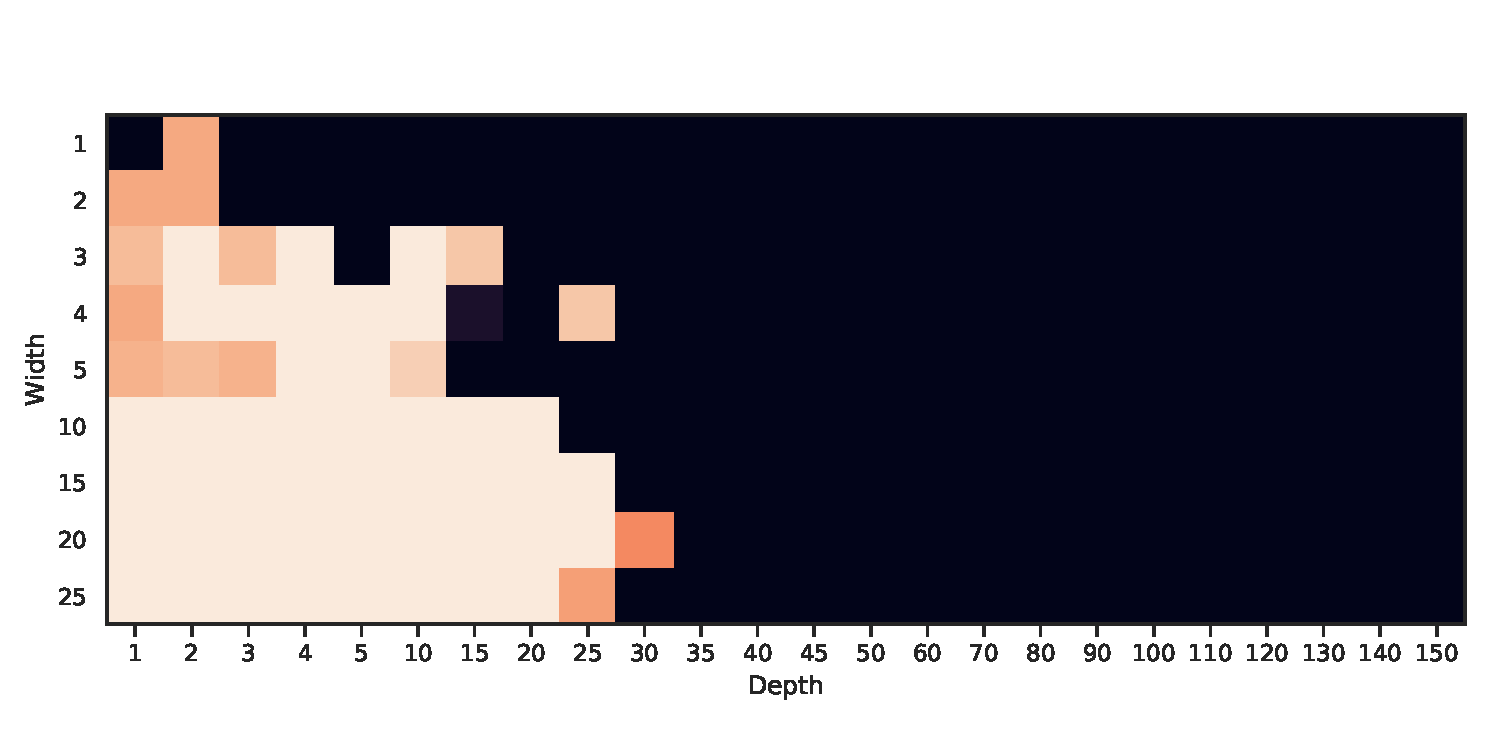
\includegraphics[width=\textwidth]{img/moons_grid/acc-relu.pdf}
        \caption{\ReLU training}
        \label{fig:moons_grid_relu}
    \end{subfigure}
    ~ %add desired spacing between images, e. g. ~, \quad, \qquad, \hfill etc. 
      %(or a blank line to force the subfigure onto a new line)
    \centering
    \begin{subfigure}[b]{0.3\textwidth}
        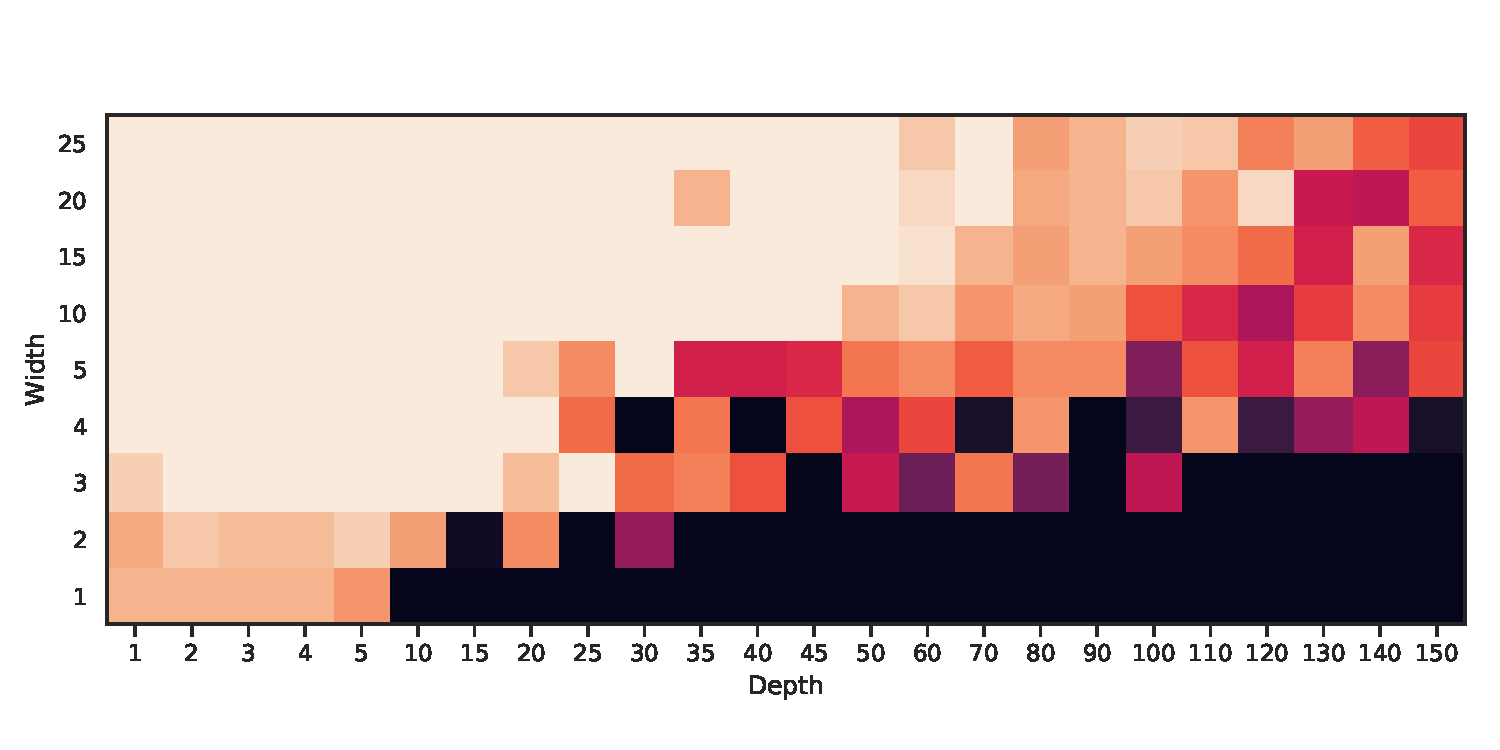
\includegraphics[width=\textwidth]{img/moons_grid/acc-relu-bn.pdf}
        \caption{\ReLUBN training}
        \label{fig:moons_grid_relubn}
    \end{subfigure}
    ~ %add desired spacing between images, e. g. ~, \quad, \qquad, \hfill etc. 
      %(or a blank line to force the subfigure onto a new line)
    \centering
    \begin{subfigure}[b]{0.3\textwidth}
        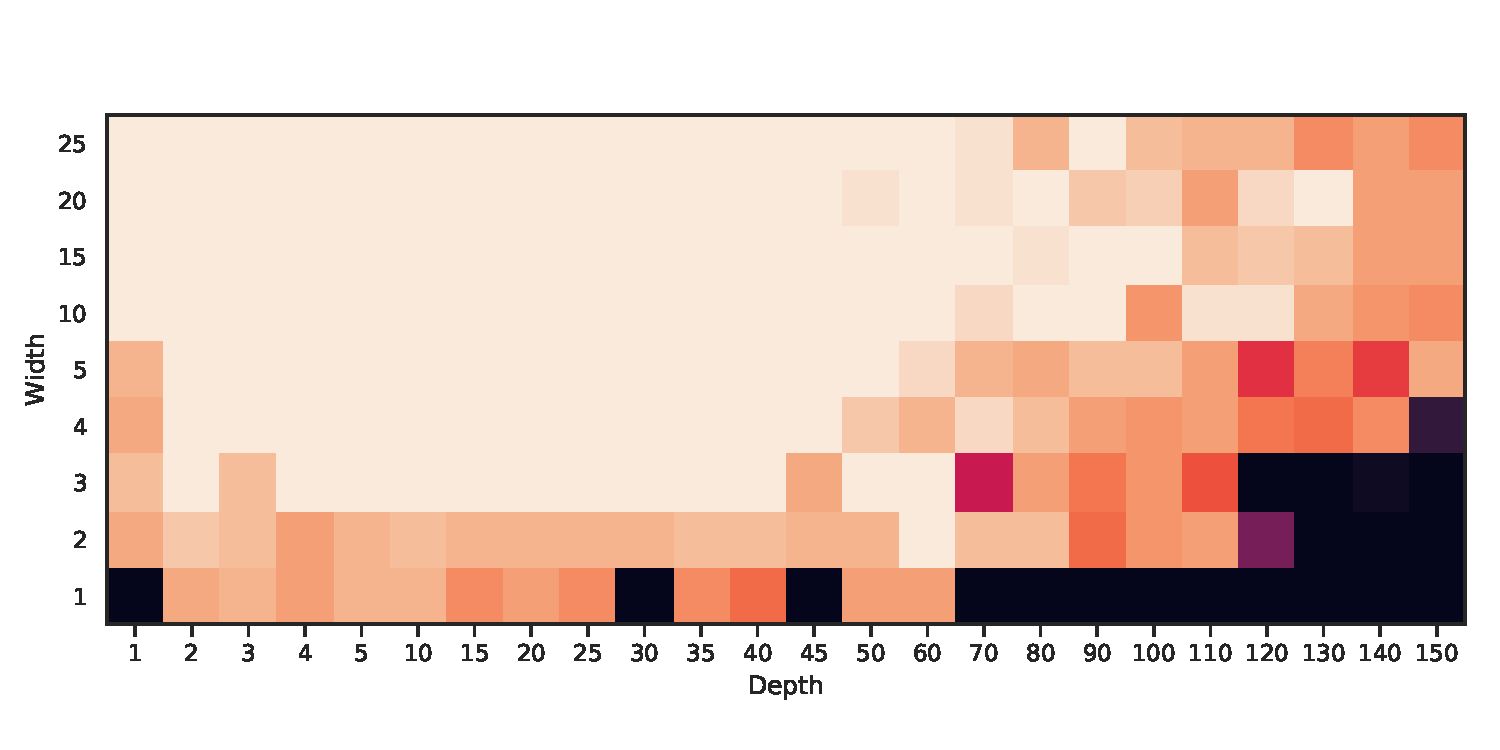
\includegraphics[width=\textwidth]{img/moons_grid/acc-sep-up-0-0001.pdf}
        \caption{\SepUnitPoint training}
        \label{fig:moons_grid_up}
    \end{subfigure}
    ~ %add desired spacing between images, e. g. ~, \quad, \qquad, \hfill etc. 
      %(or a blank line to force the subfigure onto a new line)
    \\
    \begin{subfigure}[b]{0.3\textwidth}
        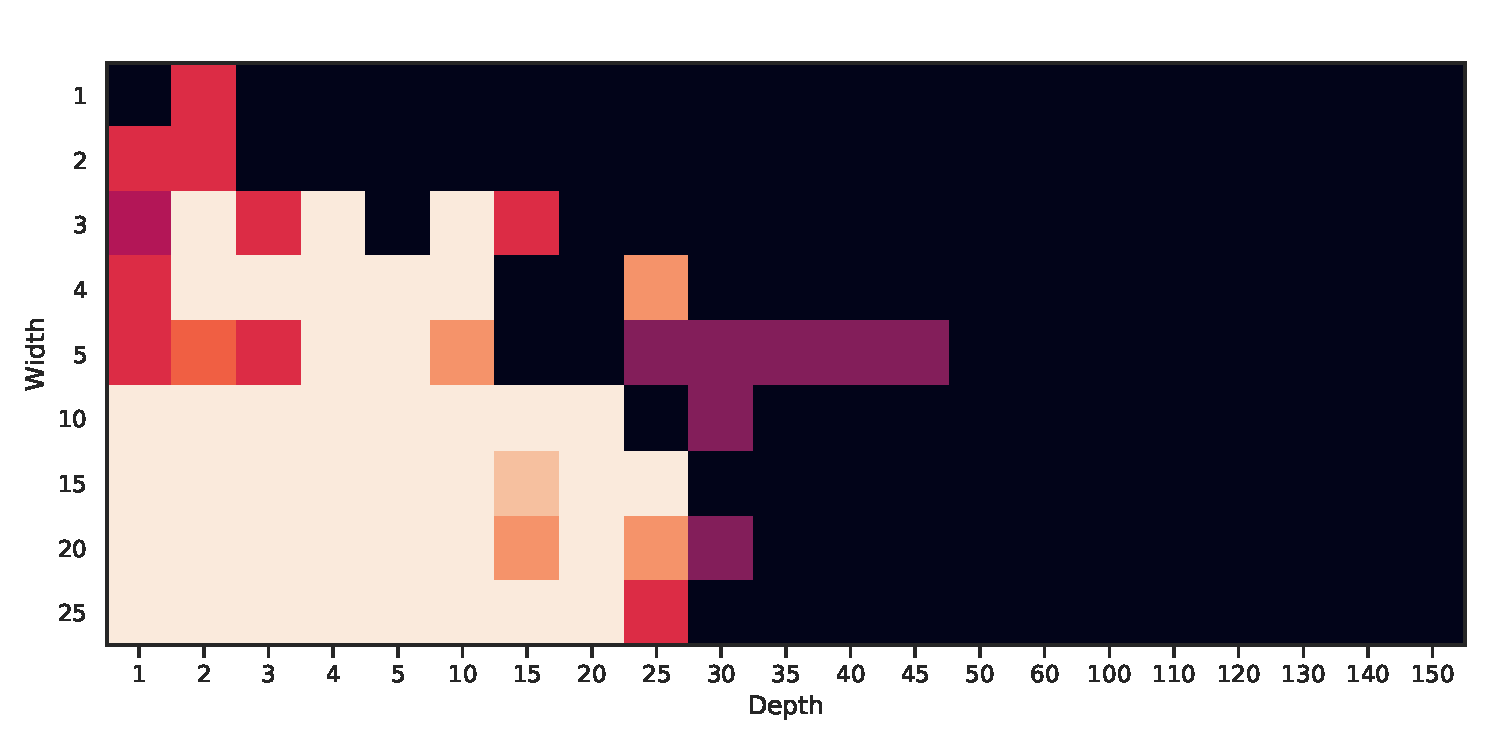
\includegraphics[width=\textwidth]{img/moons_grid/val-acc-relu.pdf}
        \caption{\ReLU validation}
        \label{fig:moons_grid_relu}
    \end{subfigure}
    ~ %add desired spacing between images, e. g. ~, \quad, \qquad, \hfill etc. 
      %(or a blank line to force the subfigure onto a new line)
    \centering
    \begin{subfigure}[b]{0.3\textwidth}
        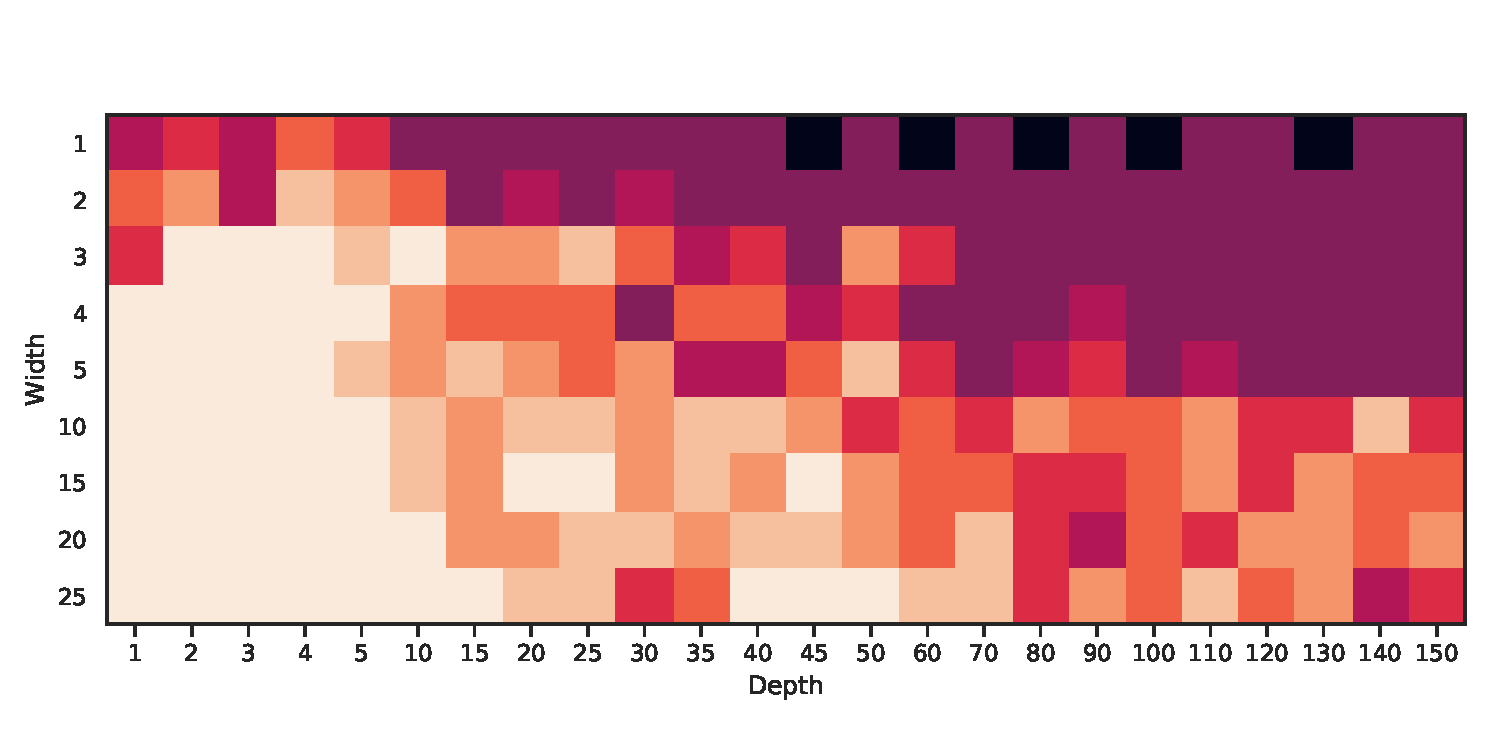
\includegraphics[width=\textwidth]{img/moons_grid/val-acc-relu-bn.pdf}
        \caption{\ReLUBN validation}
        \label{fig:moons_grid_relubn}
    \end{subfigure}
    ~ %add desired spacing between images, e. g. ~, \quad, \qquad, \hfill etc. 
      %(or a blank line to force the subfigure onto a new line)
    \centering
    \begin{subfigure}[b]{0.3\textwidth}
        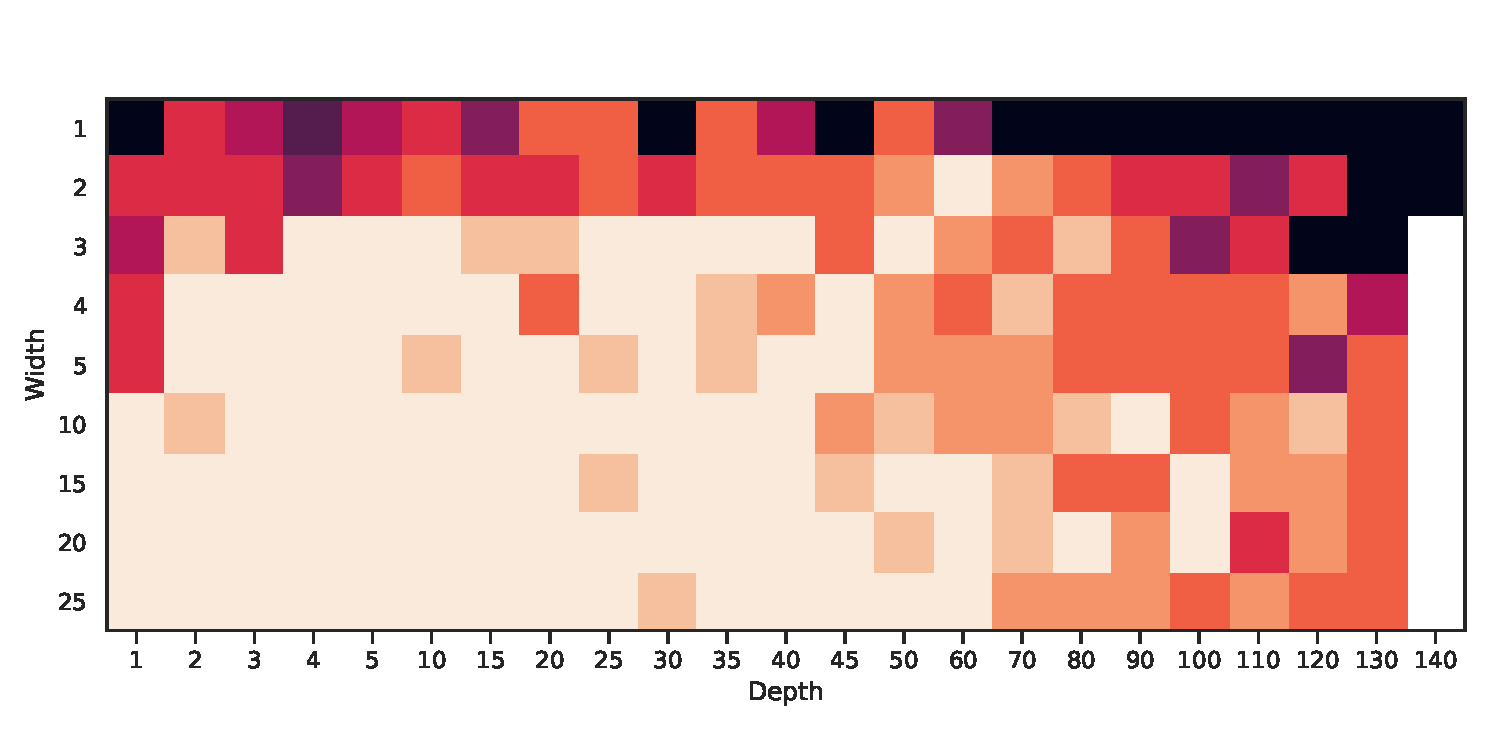
\includegraphics[width=\textwidth]{img/moons_grid/val-acc-sep-up-0-0001.pdf}
        \caption{\SepUnitPoint validation}
        \label{fig:moons_grid_up}
    \end{subfigure}
    ~ %add desired spacing between images, e. g. ~, \quad, \qquad, \hfill etc. 
      %(or a blank line to force the subfigure onto a new line)
      \\
    \begin{subfigure}[b]{0.3\textwidth}
        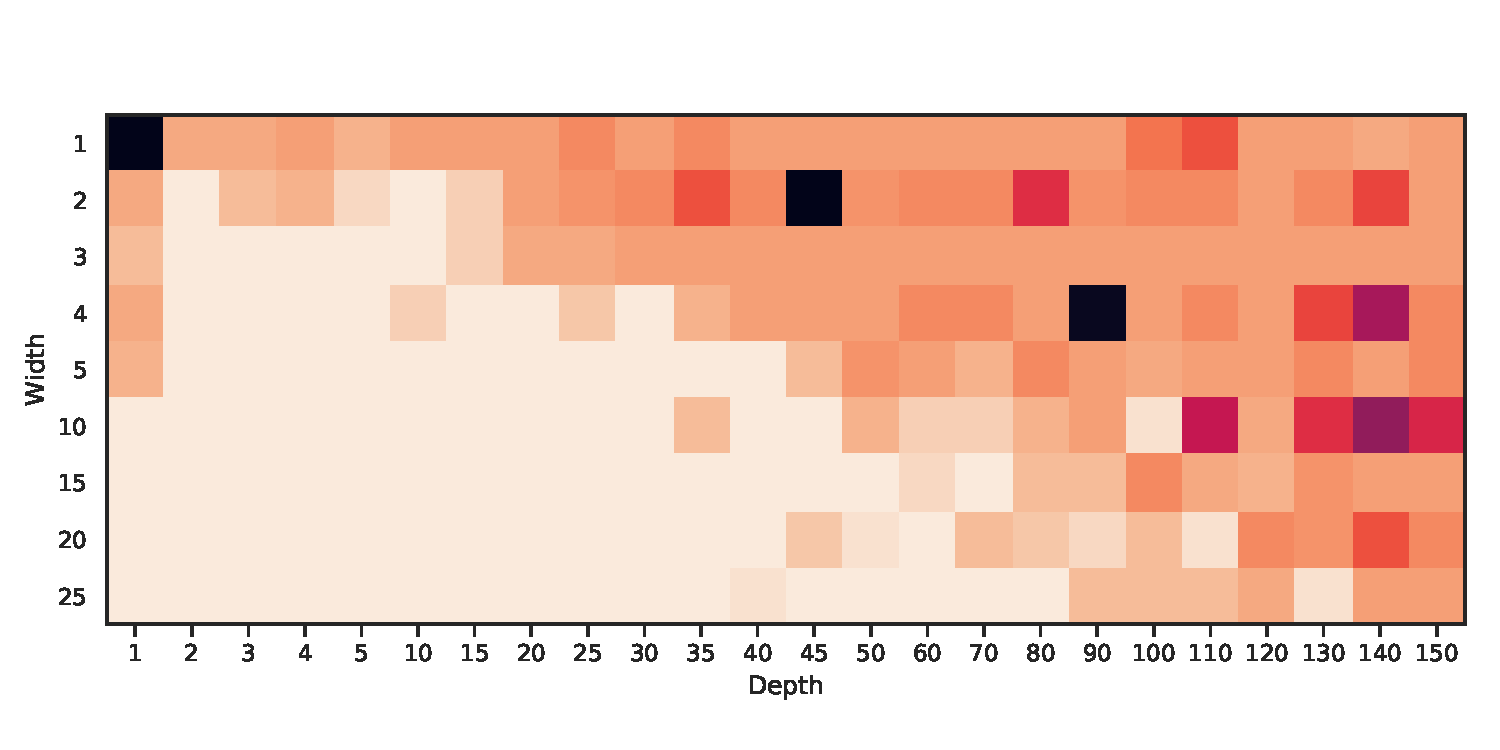
\includegraphics[width=\textwidth]{img/moons_grid/acc-sep-u-0-0001.pdf}
        \caption{\SepUnit training}
        \label{fig:moons_grid_u}
    \end{subfigure}
    ~ %add desired spacing between images, e. g. ~, \quad, \qquad, \hfill etc. 
      %(or a blank line to force the subfigure onto a new line)
    \centering
    \begin{subfigure}[b]{0.3\textwidth}
        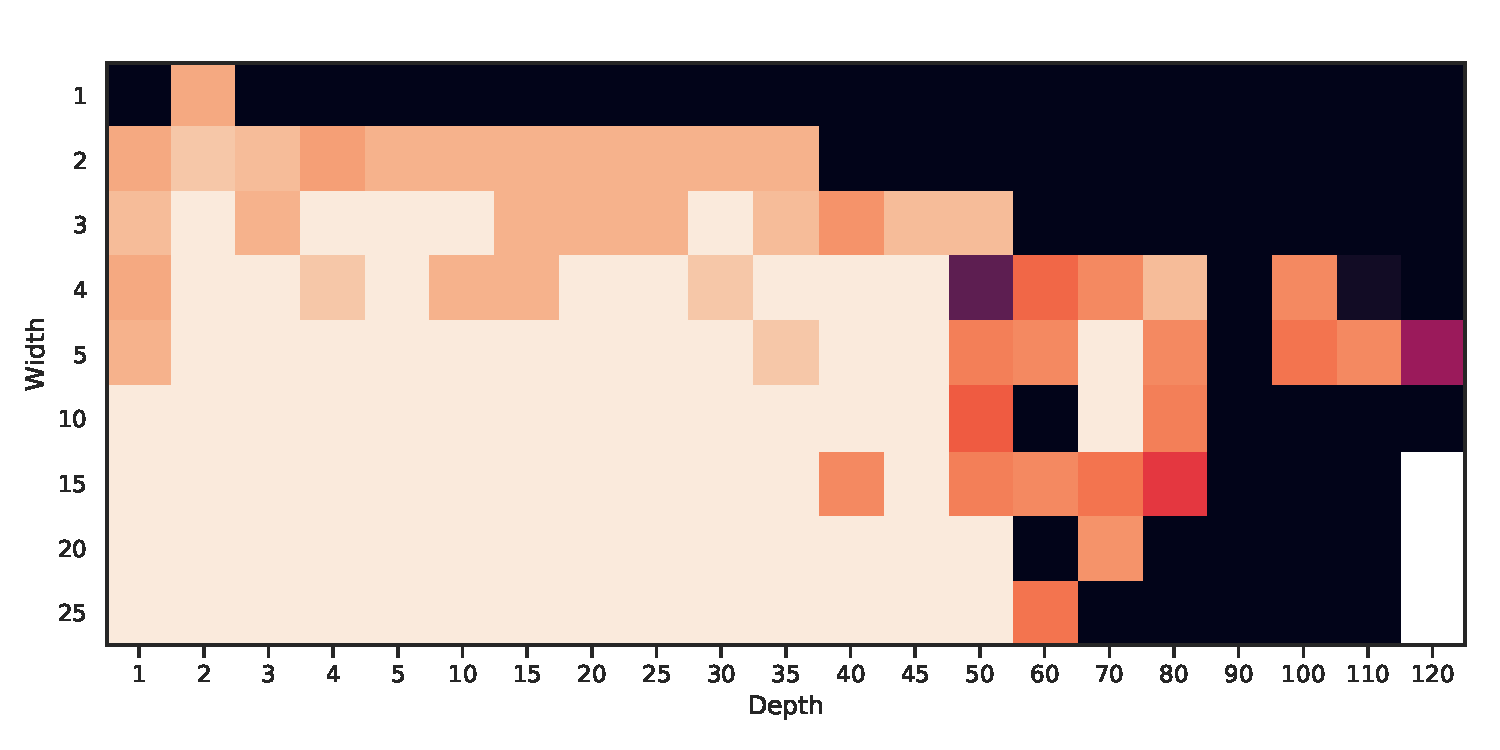
\includegraphics[width=\textwidth]{img/moons_grid/acc-sep-p-0-0001.pdf}
        \caption{\SepPoint training}
        \label{fig:moons_grid_p}
    \end{subfigure}
    ~ %add desired spacing between images, e. g. ~, \quad, \qquad, \hfill etc. 
      %(or a blank line to force the subfigure onto a new line)
    \\
    \begin{subfigure}[b]{0.3\textwidth}
        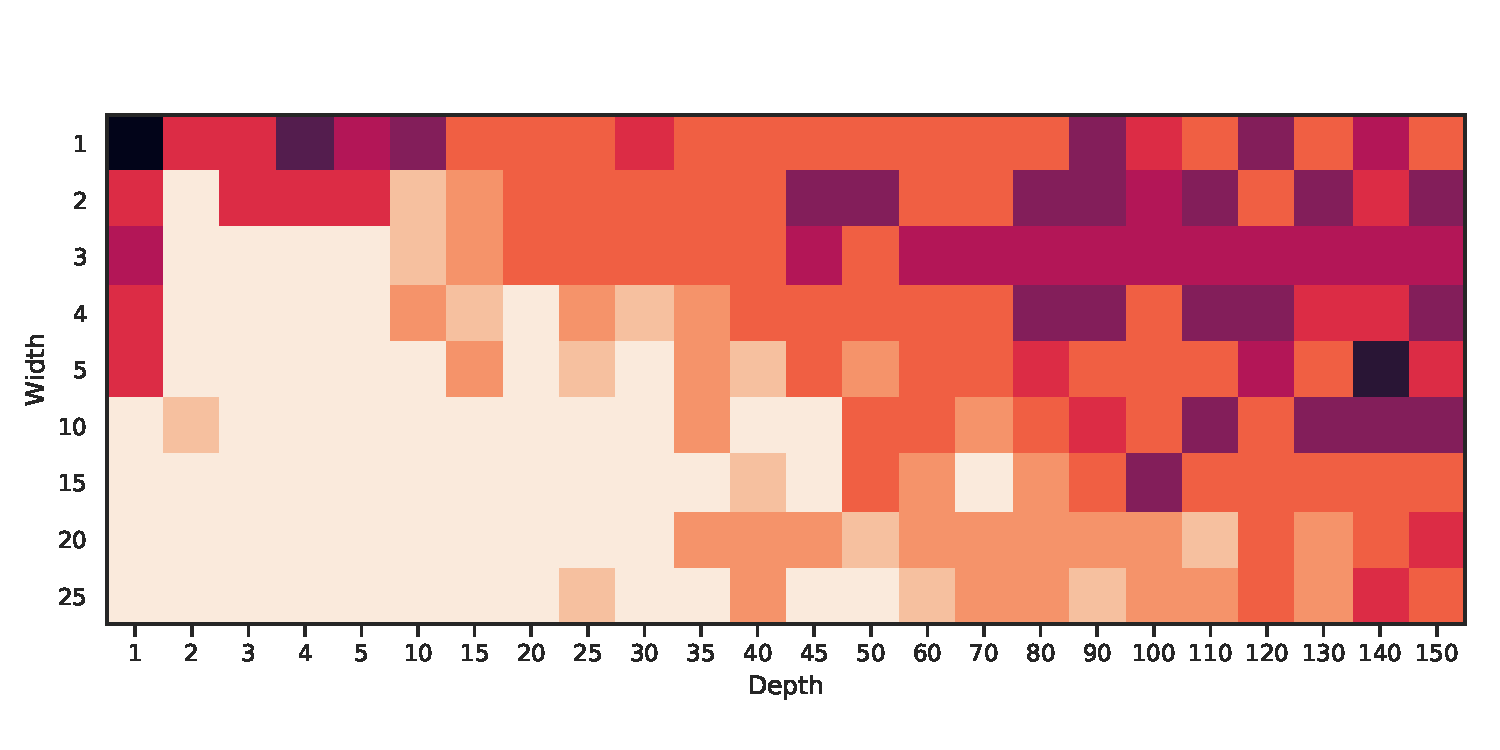
\includegraphics[width=\textwidth]{img/moons_grid/val-acc-sep-u-0-0001.pdf}
        \caption{\SepUnit validation}
        \label{fig:moons_grid_u}
    \end{subfigure}
    ~ %add desired spacing between images, e. g. ~, \quad, \qquad, \hfill etc. 
      %(or a blank line to force the subfigure onto a new line)
    \centering
    \begin{subfigure}[b]{0.3\textwidth}
        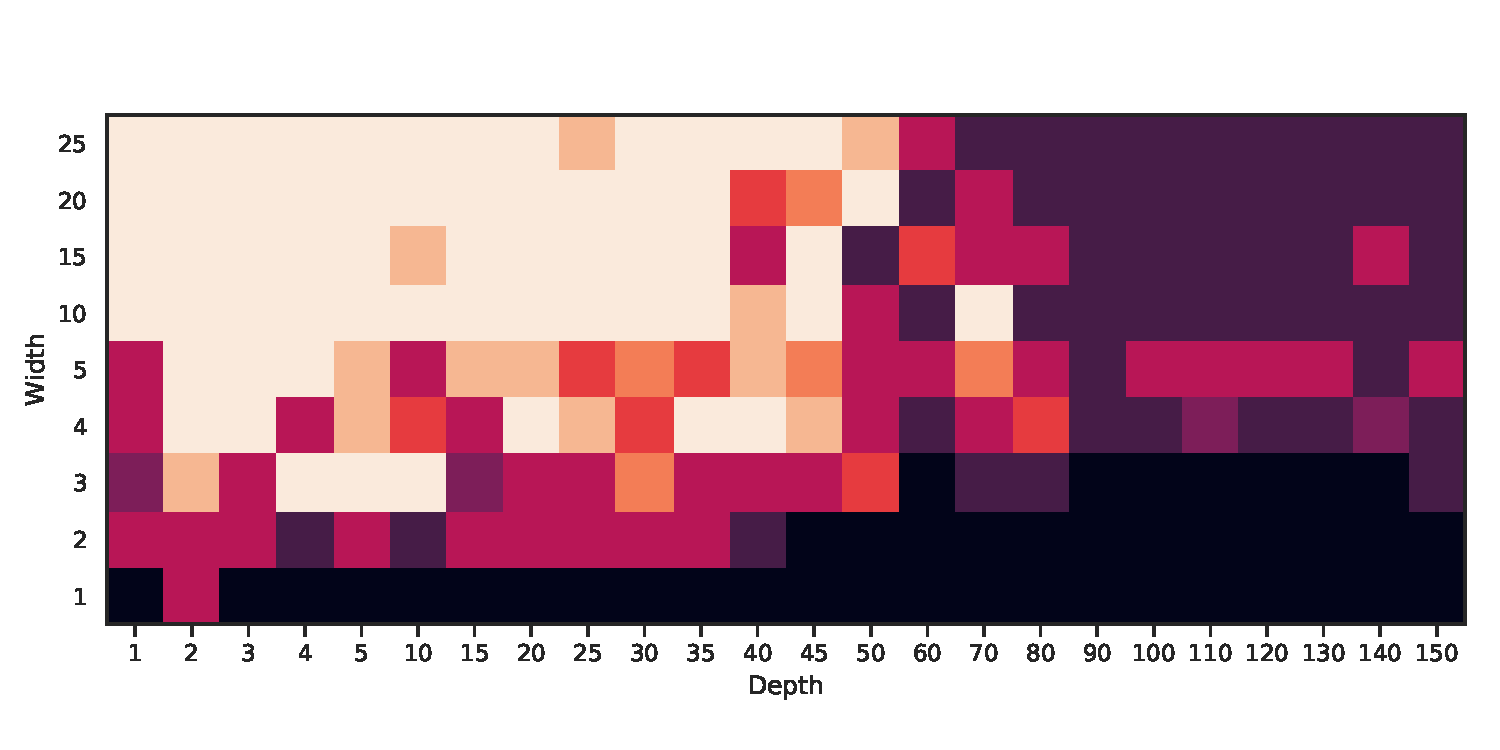
\includegraphics[width=\textwidth]{img/moons_grid/val-acc-sep-p-0-0001.pdf}
        \caption{\SepPoint validation}
        \label{fig:moons_grid_p}
    \end{subfigure}
    ~ %add desired spacing between images, e. g. ~, \quad, \qquad, \hfill etc. 
      %(or a blank line to force the subfigure onto a new line)
    
    
  \caption{Depth vs Width accuracy plot a for rectangular network using a grid (width from $2$ to $25$ and depth from $2$ to $150$),  trained using a Adam learning rate of $0.01$ in the \moons dataset. The color show the accuracy attained of each of the combinations of width and depth, the clearer the better. Notice how \ReLU, Figure \ref{fig:moons_grid_relu}, fails with networks deeper than 30 layers. In other hand, \ReLUBN, Figure \ref{fig:moons_grid_relubn}, manages to work until 70 layers deep. \SepUnitPoint,  Figure \ref{fig:moons_grid_up}, works significantly better than both, up to 120 layers. Notice how all the methods suffer from degradation from depth, which is partially alleviated by the use of greater width. This is consistent with \cite{simpnet} and \cite{densenet}. However, \SepUnitPoint is able to delay the apparition of the issue. This is especially visible when the number of units is small (from $2$ to $5$) where \ReLUBN fails to work whereas \SepUnitPoint does not. Regarding to the role of the constraint on its success, we find that \SepUnit, Figure \ref{fig:moons_grid_u}, allows the network to grow deeper, yet the accuracy can be lower following the linear decrease with the inverse of the width, which we blame on the inability of the \SepUnit constraint to address the \emph{dead point} issue. In the other hand, \SepPoint, Figure \ref{fig:moons_grid_p}, seems to perform well up to 50 layers, but it breaks down afterwards. Finally, \SepLayer , Figure \ref{fig:moons_grid_l} seems to suffer if the width is too large, performing well up to 70 layers.}
  \label{fig:moons_grid} 
\end{figure*}


\begin{figure*}
  \centering
    \begin{subfigure}[b]{0.3\textwidth}
        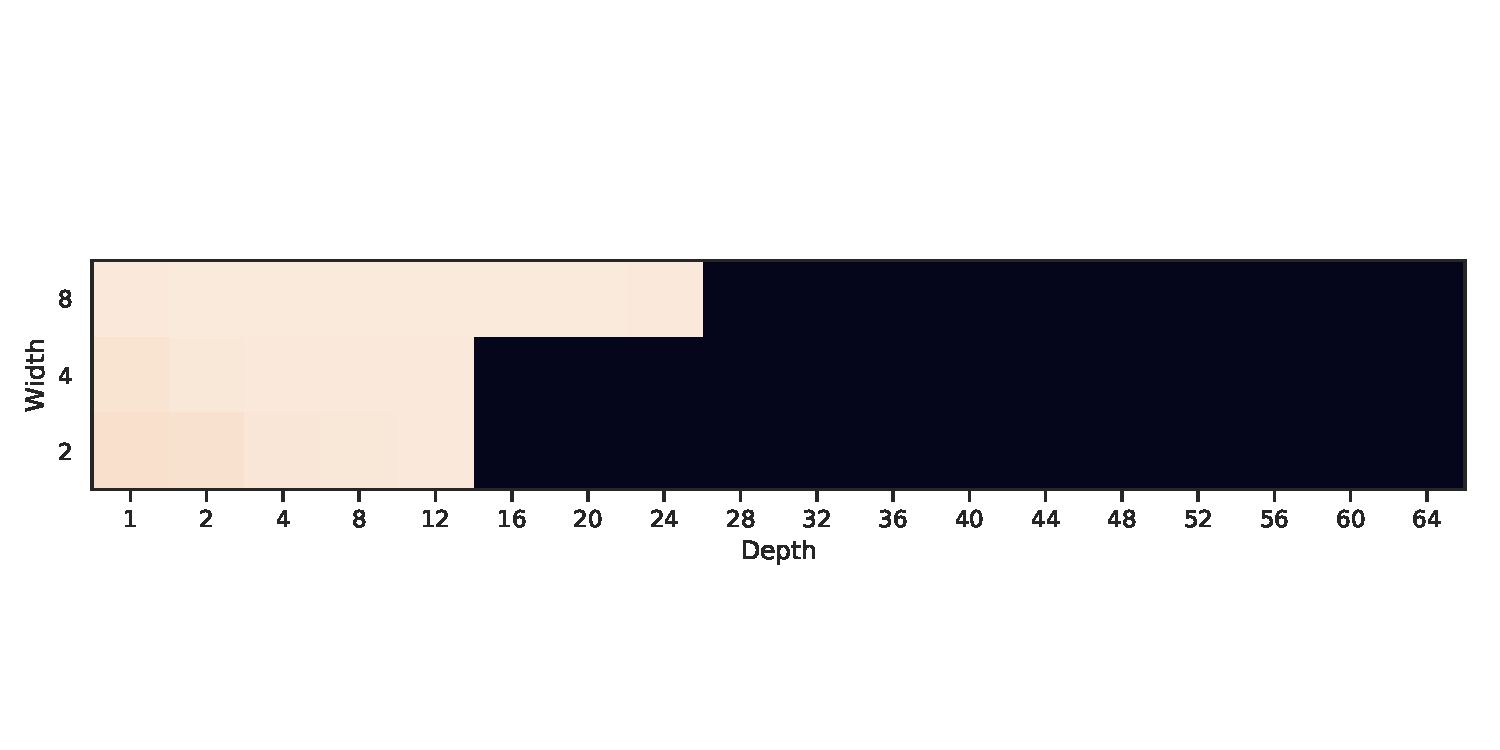
\includegraphics[width=\textwidth]{img/mnist_grid/acc-relu-ks-3x3-bs-1024.pdf}
        \caption{\ReLU}
        \label{fig:mnist_grid_relu}
    \end{subfigure}
    ~ %add desired spacing between images, e. g. ~, \quad, \qquad, \hfill etc. 
      %(or a blank line to force the subfigure onto a new line)
    \centering
    \begin{subfigure}[b]{0.3\textwidth}
        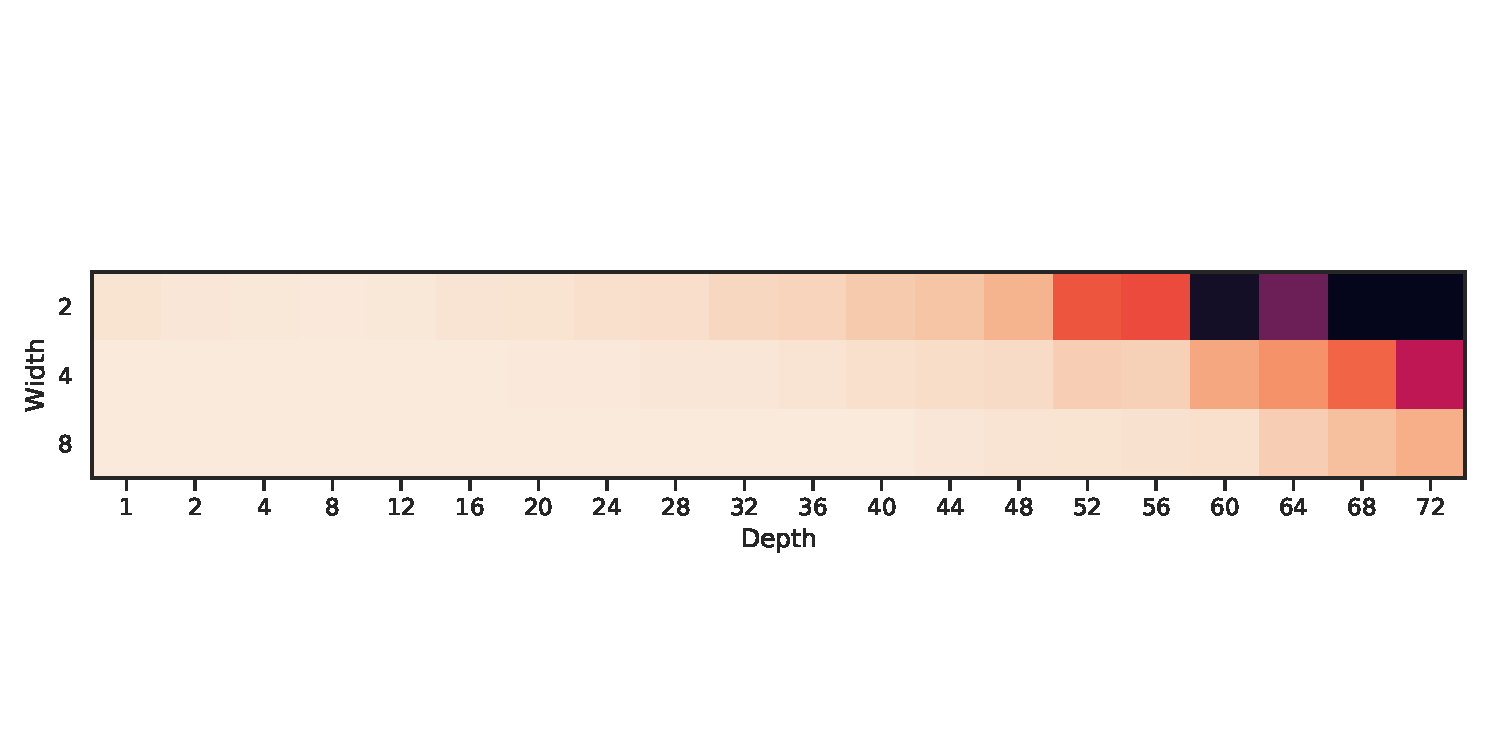
\includegraphics[width=\textwidth]{img/mnist_grid/acc-relu-bn-ks-3x3-bs-1024.pdf}
        \caption{\ReLUBN}
        \label{fig:mnist_grid_relubn}
    \end{subfigure}
    ~ %add desired spacing between images, e. g. ~, \quad, \qquad, \hfill etc. 
      %(or a blank line to force the subfigure onto a new line)
    \centering
    \begin{subfigure}[b]{0.3\textwidth}
        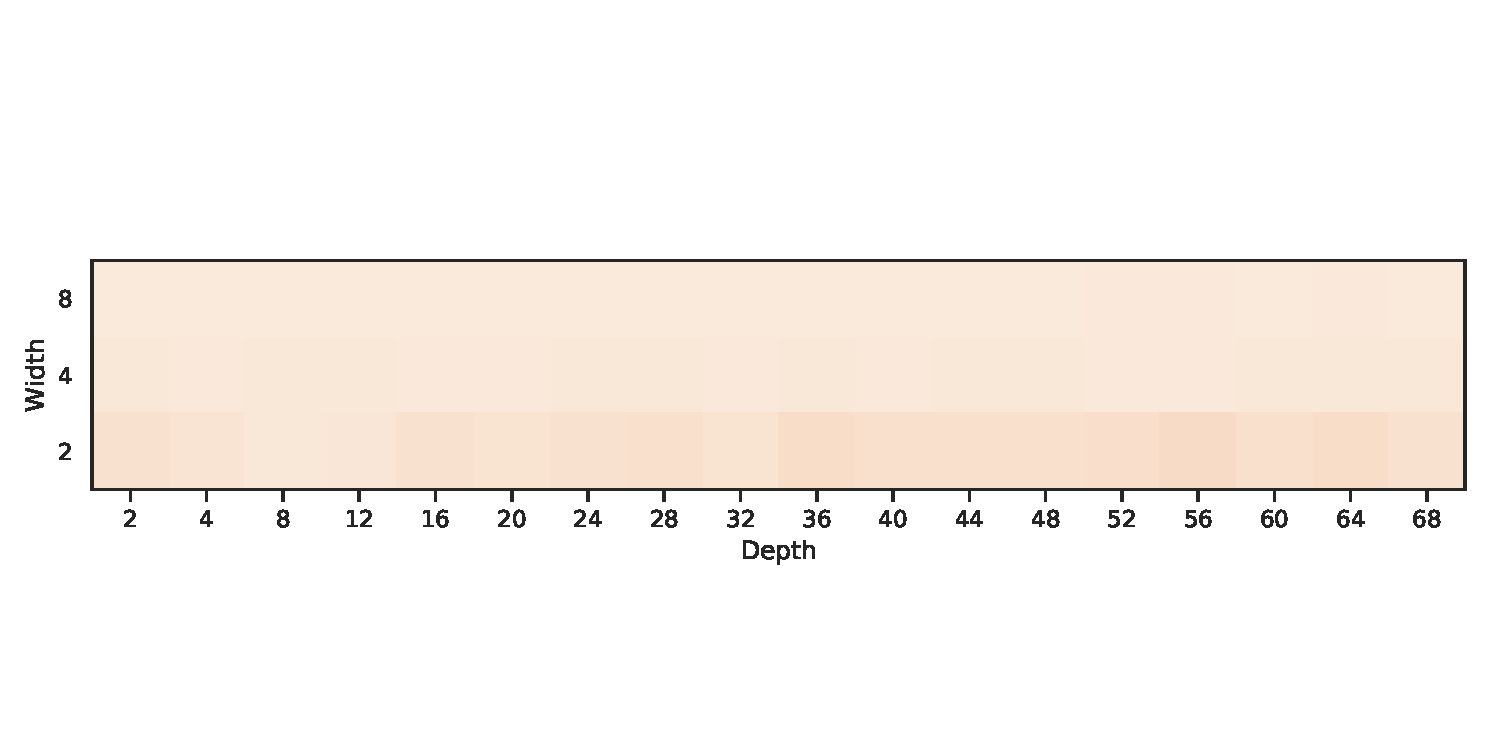
\includegraphics[width=\textwidth]{img/mnist_grid/acc-sep-up-1e-08-ks-3x3-bs-1024.pdf}
        \caption{\SepUnitPoint}
        \label{fig:mnist_grid_up}
    \end{subfigure}
    ~ %add desired spacing between images, e. g. ~, \quad, \qquad, \hfill etc. 
      %(or a blank line to force the subfigure onto a new line)
    
  \caption{Depth vs Width accuracy plot a for rectangular network using a grid (width from $2$ to $25$ and depth from $2$ to $150$),  trained using a Adam learning rate of $0.01$ in the MNIST dataset. The color show the accuracy attained of each of the combinations of width and depth, the clearer the better. Notice how \ReLU, Figure \ref{fig:mnist_grid_relu}, fails with networks deeper than 30 layers. In other hand, \ReLUBN, Figure \ref{fig:mnist_grid_relubn}, manages to work until 70 layers deep. \SepUnitPoint,  Figure \ref{fig:mnist_grid_up}, works significantly better than both, up to 120 layers. Notice how all the methods suffer from degradation from depth, which is partially alleviated by the use of greater width. This is consistent with \cite{simpnet} and \cite{densenet}. However, \SepUnitPoint is able to delay the apparition of the issue. This is especially visible when the number of units is small (from $2$ to $5$) where \ReLUBN fails to work whereas \SepUnitPoint does not.}
  \label{fig:mnist_grid} 
\end{figure*}



\begin{table*}
\begin{tabular}{llrrrrr}
\toprule
                    &    &       2  &       10 &       25 &       30 &       40 \\
\midrule
relu ks 3x3 & 10 &  0.72142 &  0.82748 &  0.09906 &  0.09880 &  0.09810 \\
relu-bn ks 3x3 & 10 &  0.90580 &  0.81764 &  0.70496 &  0.66718 &  0.59642 \\
Sep-UP 1e-08 ks 3x3 & 10 &  0.69264 &  0.79044 &  0.74344 &  0.70452 &  0.68416 \\
\bottomrule
\end{tabular}

\\
\begin{tabular}{llrrrrr}
\toprule
                    &    &      2  &      10 &      25 &      30 &      40 \\
\midrule
relu ks 3x3 & 10 &  0.5958 &  0.6052 &  0.1000 &  0.1000 &  0.1000 \\
relu-bn ks 3x3 & 10 &  0.5682 &  0.5385 &  0.5414 &  0.5328 &  0.4512 \\
Sep-UP 1e-08 ks 3x3 & 10 &  0.5874 &  0.5703 &  0.5353 &  0.5300 &  0.5320 \\
\bottomrule
\end{tabular}

\caption{}\label{tab:cifar10}
\end{table*}
\section{Conclusions}\label{sec:conclusions}
In terms of performance of the separation constraint in comparison to batchnorm as an enhancement to \ReLU networks, we find common ground with the thoughts presented by Hasanpour et al. in the \texttt{SimpNet} paper \cite{simpnet} with regards to an a-priori relation between depth and width. While Hasnpout et al. suggest that as networks grow deeper, so should the width. We provide an interpretation of it. For a rectangular network of fixed with $W$ and depth $D$, let $A_{F,X}(W,D)$ denote the accuracy reached by network $F$ (in the sense of section \ref{sec:separability}) over dataset $X$. Then the possible configurations
\\\\
We would like to remark that the Separation constraint are effective either using fully-connected or convolutional layers, see Section \ref{sec:experiments}.
\\\\
We find that although the Separation constraints enable to train deeper networks, this improvement is not absolute and eventually it fails. However, it is able to improve Batch Normalization by tranining using the minimum width twice as deep. Additionally, we find experimentally that it also induces unstabilities during training which display interesting properties like increasingly complex but smoother boundaries which indeed require of further research.
\\\\
However, further inquiry into the interaction between constraint loss and main loss beyond parameter $\lambda$ is needed, alongside with experiments regarding other losses besides cross-entropy. In addition,  the use of the separation constraints in other types of layers such as LSTM \cite{lstm} or transformers \cite{transformer}\cite{transformer2} is yet to be performed, in order to explore other types of tasks like regression, unsupervised learning \cite{embedding}, graph \cite{graph} or generation \cite{gan,vae}. Morever, more challenging datasets are definitely in need of revision.
\\\\

% 4.1
While the separation constraints prevent the vanishing gradient, the \emph{exploding gradient} remains at large. Notice that constraint introduction places \emph{lower bounds} on the magnitude of the pre-activation values, but does not place upper bounds. This could be solved introducing additional constraints forcing them. 








%%%%%%%%%%%%%%%%%%%%%%%%%%%%%%%%%%%%%%%% BIBLIOGRAPHY %%%%%%%%%%%%%%%%%%%%%%%%%%%%%%%%%%%%%%%%%%%%%%%%%%%%%%%%%%%%%%%%%
{\small
\bibliographystyle{ieee}
\bibliography{references}
%\nocite{*}
}

\end{document}

